\documentclass[12pt]{report}

\usepackage[language=english, type=bachelor]{style}

\usepackage{booktabs}
\usepackage{array}
\usepackage{tabularx}
\usepackage{colortbl}
\usepackage{makecell}
\usepackage{ragged2e}
\usepackage{caption}
\usepackage{subcaption}
\usepackage{float}
\usepackage{amsmath}
\usepackage{amssymb}
\usepackage{enumitem}
\usepackage{listings}
\usepackage{xcolor}

\definecolor{codegray}{rgb}{0.5,0.5,0.5}
\definecolor{codepurple}{rgb}{0.58,0,0.82}
\definecolor{codeblue}{rgb}{0.13,0.29,0.53}
\definecolor{codegreen}{rgb}{0,0.5,0}
\definecolor{backcolour}{rgb}{0.97,0.97,0.97}

\lstdefinestyle{pythonstyle}{
    backgroundcolor=\color{backcolour},
    commentstyle=\color{codegreen}\itshape,
    keywordstyle=\color{codeblue}\bfseries,
    stringstyle=\color{codepurple},
    basicstyle=\ttfamily\footnotesize,
    breakatwhitespace=false,
    breaklines=true,
    captionpos=b,
    keepspaces=true,
    numbers=left,
    numbersep=8pt,
    numberstyle=\tiny\color{codegray},
    showspaces=false,
    showstringspaces=false,
    showtabs=false,
    tabsize=4,
    frame=single,
    framerule=0.4pt,
    rulecolor=\color{gray!40},
    xleftmargin=16pt,
    xrightmargin=4pt,
}
\lstdefinestyle{pseudostyle}{
    backgroundcolor=\color{backcolour},
    basicstyle=\ttfamily\footnotesize,
    keywordstyle=\bfseries,
    commentstyle=\color{codegreen}\itshape,
    breakatwhitespace=false,
    breaklines=true,
    captionpos=b,
    keepspaces=true,
    showspaces=false,
    showstringspaces=false,
    frame=single,
    framerule=0.4pt,
    rulecolor=\color{gray!40},
    xleftmargin=8pt,
    xrightmargin=4pt,
    mathescape=true,
}
\renewcommand{\lstlistingname}{Listing}

\usepackage{tikz}
\usetikzlibrary{arrows.meta, positioning, shapes.geometric, backgrounds, fit, decorations.markings, calc, shadows.blur}
\usepackage{cleveref}

\usepackage{fancyhdr}
\pagestyle{fancy}
\lhead{}
\chead{}
\renewcommand{\headrulewidth}{0.2pt}
\renewcommand{\footrulewidth}{0.2pt}

\begin{document}

\specialization{Computer Science}
\title{Structural Context Retrieval for AI Coding Agents via Weighted Personalized PageRank on Code Dependency Graphs}
\author{Toma Alexandru-Mihai}
\supervisor{Dr. Arthur Molnar}

\hypersetup{pageanchor=false}
\maketitle
\hypersetup{pageanchor=true}

\cleardoublepage
\pagenumbering{roman}

\tableofcontents

\newpage
\pagenumbering{arabic}

% =============================================================================
% Chapter 1: Introduction
% =============================================================================

\chapter{Introduction}
\label{ch:introduction}

Large Language Models (LLMs) have made AI coding agents useful for more than isolated code completion. Agents can now inspect files, propose patches, and run tests, but their success still depends on a simple prerequisite: they must see the right code. Repository-scale tasks make this difficult. A bug report may describe a symptom in natural language, while the relevant implementation is spread across imports, calls, and inheritance relationships that are not visible to text search alone.

This thesis introduces CodeGraph, a hybrid retrieval system for repository-level code navigation. CodeGraph parses Python repositories into a dependency graph, selects seed entities from a task description, and uses Personalized PageRank to rank structurally related code. The central claim is that lexical matching places the search in the right region of the codebase, and graph propagation ranks structurally related code once that region is reached. Lexical signals identify where the search can begin; graph propagation identifies which connected code entities are likely to matter.

% =============================================================================
\section{Motivation}
\label{sec:motivation}
% =============================================================================

Code retrieval methods treat each file as an independent document, but codebases are not collections of independent documents. They are connected systems where functionality is distributed across imports, calls, and inheritance hierarchies. A task described in natural language may require understanding code that is structurally close but textually distant, linked by dependency chains that text search cannot follow.

The primary bottleneck is Seed Extraction: translating an ambiguous task description into useful starting points inside the code graph. If no seed lands near the relevant subsystem, even a strong ranking algorithm has little useful signal to propagate. If the seed set contains a mix of correct and noisy matches, graph structure can still help by amplifying the region where independent signals converge. CodeGraph is designed around this division of labor.

% =============================================================================
\section{Research Objectives and Original Contributions}
\label{sec:objectives}
% =============================================================================

This research develops CodeGraph, a graph-based retrieval system for AI coding agents. The specific contributions are:

\begin{enumerate}
    \item A Tree-sitter-based parsing pipeline that extracts calls, imports, and inheritance relationships from Python source code to construct a weighted dependency graph.
    \item A hybrid retrieval engine that pairs lexical matching with Personalized PageRank propagation, producing deterministic, structure-aware rankings of codebase entities.
    \item An MCP server for AI agent integration and a CLI tool for direct use.
    \item A visualization application for exploring code dependency graphs and understanding retrieval results.
    \item A comprehensive evaluation on SWE-bench Lite (300 real software issues), demonstrating 74.0\% Recall@10 and a 24.3 percentage point improvement over the BM25 baseline.
\end{enumerate}

% =============================================================================
\section{Thesis Structure}
\label{sec:roadmap}
% =============================================================================

The thesis is organized as a progression from problem definition to system validation. Chapters 2 and 3 establish the foundations: Chapter 2 provides the technical background on static analysis and graph-based ranking while surveying related work, and Chapter 3 presents the architectural design of CodeGraph and the theoretical basis for graph-based relevance propagation. Chapters 4 and 5 describe the system and its evaluation: Chapter 4 details the implementation and algorithmic choices, and Chapter 5 reports results on SWE-bench Lite. Chapters 6 and 7 interpret these findings: Chapter 6 discusses the broader implications for AI coding agents, and Chapter 7 summarizes contributions and outlines future research directions.

\paragraph{Declaration of AI Assistance.} During the preparation of this work the author used Claude in order to refine the vocabulary for academic style. After using this tool/service, the author reviewed and edited the content as needed and takes full responsibility for the content of the thesis.


% ============================================================
%  Chapter 2 — Background and Related Work
% ============================================================
\chapter{Background and Related Work}
\label{chap:background}

This chapter identifies the fundamental constraints of code retrieval for LLM-based agents. We define the retrieval problem, establish its requirements, and survey established methodological families.

% ============================================================
\section{Code Retrieval for AI Agents}
\label{sec:code-retrieval}
% ============================================================

LLM-based coding agents face a fundamental selection problem: given a natural language task description and a large code repository, which source files should the agent examine? This section defines this retrieval problem, establishes its constraints, and surveys three classes of methods---sparse, dense, and graph-based---that represent increasingly structural approaches to solving it.

% ------------------------------------------------------------
\subsection{The Retrieval Problem}
\label{sec:retrieval-problem}
% ------------------------------------------------------------

Transformer-based language models process a fixed-length token sequence at inference time. For current production models, this limit ranges from 32{,}000 to 200{,}000 tokens~\cite{gpt4,claude3}, while a moderately sized Python repository---Django being a representative example---contains several million tokens of source code. An agent operating on such a repository must therefore select a small subset of files, typically 5--20, that is likely to contain the code relevant to the task at hand~\cite{yang2024swebench}.

This selection problem has an asymmetric cost structure. A false negative---failing to retrieve a file that the agent must modify---renders the task unsolvable regardless of the agent's subsequent reasoning quality. A false positive---retrieving an irrelevant file---incurs only a noise cost: it consumes context budget but does not prevent a correct solution. This asymmetry makes retrieval fundamentally \emph{recall-oriented}: the primary measure of retrieval quality is whether the relevant files appear within the top-$k$ results, rather than the precision of the entire retrieved set.

% ------------------------------------------------------------
\subsection{Retrieval-Augmented Generation for Code}
\label{sec:rag}
% ------------------------------------------------------------

Retrieval-augmented generation (RAG)~\cite{lewis2020rag} addresses the context window limitation by treating the repository as an external knowledge base. A typical RAG pipeline first retrieves candidate code entities, then uses an LLM to reason over the retrieved context. The quality of generation is strictly bounded by retrieval: an LLM cannot produce a correct fix for code it was not shown.

RAG for code faces a fundamental challenge: bridging the modal gap between natural language task descriptions and structured source code. A bug report uses high-level, ambiguous prose, while the retrieval targets are syntax-constrained code entities interconnected through explicit dependencies. Surface-level text similarity often fails to identify the relevant code. Recent empirical work confirms that retrieval quality, rather than reasoning capacity, is the dominant bottleneck in agent performance~\cite{yang2024swebench}. Evaluations on benchmarks such as SWE-bench demonstrate that agents with targeted retrieval mechanisms outperform those given larger but unfocused context~\cite{yang2024swebench}.

% ------------------------------------------------------------
\subsection{Sparse, Dense, and Graph-Based Retrieval}
\label{sec:retrieval-families}
% ------------------------------------------------------------

We now examine three classes of retrieval methods in turn, analyzing their strengths and fundamental limitations.
The key characteristics of these families are summarized in \cref{tab:retrieval-comparison}, and their respective conceptual workflows are illustrated in \cref{fig:retrieval-flow}.

\paragraph{Sparse retrieval.}
Sparse retrieval methods compute relevance as a weighted term overlap between the query and the indexed code tokens. BM25~\cite{bm25}, the dominant method in this class, scores each document using term frequency, inverse document frequency, and a saturation function that prevents overfitting to high-frequency terms. Sparse methods require no learned parameters, scale to large corpora, and produce interpretable scores. Their principal limitation is lexical sensitivity: relevance is measured at the token level, so a query term and a code identifier that express the same concept but differ in surface form will not match. In source code, this is a pervasive problem. Identifiers frequently combine multiple semantic units into a single compound token---such as \texttt{SQLCompiler}, \texttt{get\_absolute\_url}, or \texttt{BaseHasher}---using camelCase or underscore conventions. A query mentioning "SQL compilation" does not match the token \texttt{SQLCompiler} under atomic tokenization. Sparse methods are therefore most effective when the vocabulary of the task description closely mirrors the vocabulary of the relevant source code, and degrade when it does not.

\paragraph{Dense retrieval.}
Dense retrieval methods encode queries and code entities into a shared continuous vector space and rank candidates by cosine similarity. Models such as CodeBERT~\cite{codebert}, GraphCodeBERT~\cite{graphcodebert}, and UniXcoder~\cite{unixcoder} are trained on large code corpora to align natural language descriptions with code representations, enabling matching that is robust to vocabulary variation and paraphrase. However, dense methods have three limitations for repository-scale retrieval. First, they compute similarity from token sequences alone and have no structural awareness: the score assigned to a candidate file is determined entirely by its textual content, without regard to which modules it imports, which functions it calls, or which components depend on it. Second, achieving competitive performance typically requires fine-tuning on domain-specific code--query pairs, which may not be available for every repository or language. Third, embedding similarity scores are opaque: there is no principled way to trace why a specific candidate received a high score, making it difficult to diagnose retrieval failures or improve the system systematically.

\paragraph{Graph-based retrieval.}
Graph-based retrieval methods represent code relationships as edges in a typed directed graph and propagate relevance from query-matched seed entities to structurally connected entities. Unlike sparse and dense methods, which score candidates independently, graph-based methods model relevance as flowing along structural connections between code entities. Recent work demonstrates the effectiveness of this approach. GraphCoder~\cite{liu2024graphcoder} captures call and data-flow relationships through a code context graph to enhance repository-level code completion. Athale and Vaddina~\cite{athale2025knowledge} construct a knowledge graph over repository structure and use graph queries to retrieve context for LLM-based generation. CodexGraph~\cite{liu2024codexgraph} further demonstrates the utility of bridging LLMs and code repositories via graph databases. These systems use sparse retrieval to identify seed nodes in a code dependency graph, then apply graph traversal or ranking algorithms (such as Personalized PageRank) to reach structurally relevant entities.

\begin{table}[H]
    \centering
    \small
    \caption{Comparison of code retrieval methodologies along key performance and implementation dimensions.}
    \label{tab:retrieval-comparison}
    \renewcommand{\arraystretch}{1.6}
    \begin{tabularx}{\textwidth}{@{} >{\RaggedRight\bfseries}p{2.4cm} >{\RaggedRight\arraybackslash}X >{\RaggedRight\arraybackslash}X >{\RaggedRight\arraybackslash}X @{}}
        \toprule
        & \textbf{Sparse} & \textbf{Dense} & \textbf{Graph-based} \\
        \midrule
        Representative systems & BM25, TF-IDF & CodeBERT, UniXcoder & GraphCoder, RANGER, GRACE \\
        Input signal & Term overlap & Vector similarity & Graph structure \\
        Structural awareness & None & None & Explicit (calls, imports, inheritance) \\
        Key strength & Fast, interpretable, no training & Vocabulary-robust, handles paraphrase & Recovers structurally coupled entities \\
        Key failure mode & Lexical mismatch (\texttt{SQLCompiler} vs. "SQL compilation") & Ignores dependency structure; opaque scores & Bounded by seed quality \\
        Training required & None & Fine-tuning on code--query pairs & None for retrieval; requires graph construction \\
        \bottomrule
    \end{tabularx}
\end{table}

\begin{figure}[H]
    \centering
    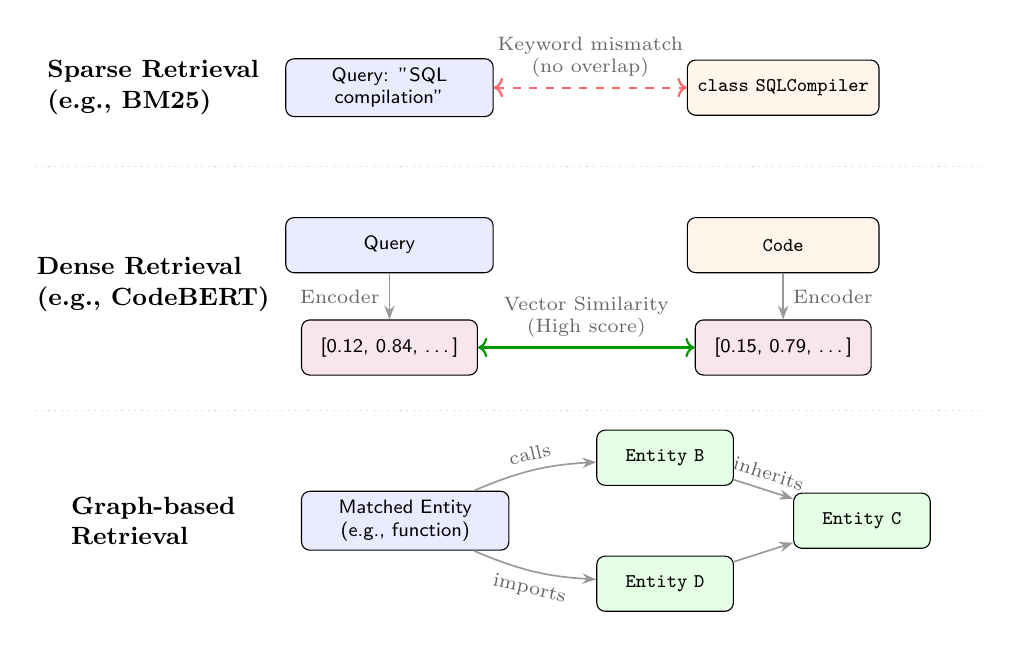
\begin{tikzpicture}[
            box/.style={draw, rectangle, rounded corners=3pt, fill=blue!8, text width=2.4cm, align=center, minimum height=0.7cm, font=\scriptsize\sffamily},
            codebox/.style={draw, rectangle, rounded corners=3pt, fill=orange!8, text width=2.2cm, align=center, minimum height=0.7cm, font=\scriptsize\ttfamily},
            arrow/.style={-{Stealth[length=5pt]}, semithick, draw=gray!80},
            lbl/.style={font=\scriptsize, align=center, text=gray!80!black},
            title/.style={font=\small\bfseries, align=left}
        ]

        % --- Sparse ---
        \node[title] (sparse_title) at (-3, 3.5) {Sparse Retrieval\\(e.g., BM25)};
        \node[box] (sq) at (0, 3.5) {Query: "SQL compilation"};
        \node[codebox] (sc) at (5, 3.5) {class SQLCompiler};
        \draw[<->, dashed, thick, draw=red!60] (sq) -- node[lbl, above] {Keyword mismatch\\(no overlap)} (sc);

        % --- Dense ---
        \node[title] (dense_title) at (-3, 1) {Dense Retrieval\\(e.g., CodeBERT)};
        \node[box] (dq) at (0, 1.5) {Query};
        \node[codebox] (dc) at (5, 1.5) {Code};
        \node[box, fill=purple!10, text width=2.0cm] (dvq) at (0, 0.2) {[0.12, 0.84, \dots]};
        \node[box, fill=purple!10, text width=2.0cm] (dvc) at (5, 0.2) {[0.15, 0.79, \dots]};
        \draw[arrow] (dq) -- node[lbl, left] {Encoder} (dvq);
        \draw[arrow] (dc) -- node[lbl, right] {Encoder} (dvc);
        \draw[<->, thick, draw=green!60!black] (dvq) -- node[lbl, above] {Vector Similarity\\(High score)} (dvc);

        % --- Graph-based ---
        \node[title] (graph_title) at (-3, -2) {Graph-based\\Retrieval};
        \node[box] (gq) at (0.2, -2) {Matched Entity\\(e.g., function)};
        
        \node[codebox, text width=1.5cm, fill=green!10] (n1) at (3.5, -1.2) {Entity B};
        \node[codebox, text width=1.5cm, fill=green!10] (n2) at (6, -2) {Entity C};
        \node[codebox, text width=1.5cm, fill=green!10] (n3) at (3.5, -2.8) {Entity D};

        \draw[arrow] (gq) to[bend left=10] node[lbl, above, sloped] {calls} (n1);
        \draw[arrow] (gq) to[bend right=10] node[lbl, below, sloped] {imports} (n3);
        \draw[arrow] (n1) -- node[lbl, above, sloped] {inherits} (n2);
        \draw[arrow] (n3) -- (n2);
        
        % Background separator lines
        \draw[dotted, draw=gray!40] (-4.5, 2.5) -- (7.5, 2.5);
        \draw[dotted, draw=gray!40] (-4.5, -0.6) -- (7.5, -0.6);

    \end{tikzpicture}
    \caption{Conceptual retrieval workflows. Sparse methods rely on keyword matching; Dense methods leverage semantic embeddings; Graph-based methods traverse structural dependencies to recover coupled code entities.}
    \label{fig:retrieval-flow}
\end{figure}

\chapter{System Design and Methodology}
\label{chap:design}


% =============================================================================
% Chapter 4: Implementation
% =============================================================================

\chapter{Implementation}
\label{ch:implementation}

% =============================================================================
\section{System Architecture}
\label{sec:system-architecture}
% =============================================================================

This chapter translates the architectural blueprint established in \cref{ch:design} into a working implementation. It traces the full pipeline from raw source files on disk to ranked code context delivered to an AI agent. The objective is to detail how the theoretical constructs (static parsing, two-pass resolution, and structural ranking) are realized in software, ensuring the system operates reliably and efficiently under the constraints of sub-second query latency.

The system is organized into distinct, sequential components. First, the parser scans the repository and extracts structural elements. Next, the resolver links these elements together. The resulting data is loaded into a graph database. When an AI agent requests context, the ranking engine traverses this database to find the most relevant code. Finally, the interface layer packages these results and delivers them to the agent.

\begin{figure}[htbp]
    \centering
    \resizebox{\textwidth}{!}{%
    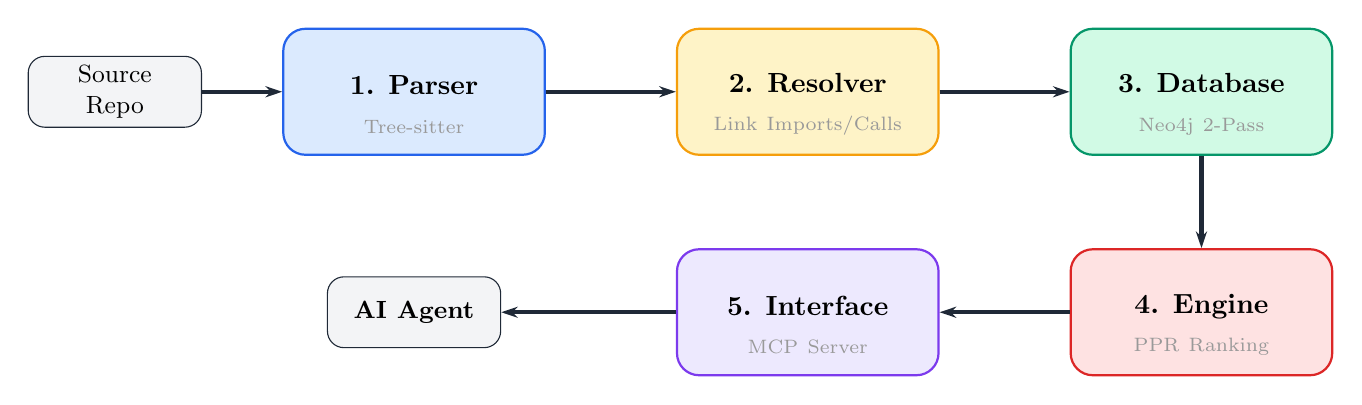
\begin{tikzpicture}[
            % Component boxes
            stage/.style={draw, rounded corners=8pt,
                    minimum width=3.2cm, minimum height=1.6cm,
                    text width=2.9cm, align=center,
                    line width=0.8pt, inner sep=6pt},
            % Number badge
            badge/.style={circle, minimum size=18pt, inner sep=0pt,
                    font=\footnotesize\bfseries, text=white, line width=0pt},
            % Main flow arrow
            arr/.style={-{Stealth[length=6pt, width=4pt]}, line width=1.5pt,
                    color={rgb,255:red,31;green,41;blue,55}},
            % Data labels
            datalabel/.style={font=\scriptsize\itshape, color={rgb,255:red,107;green,114;blue,128},
                    align=center, inner sep=2pt}
        ]

        % 1. Parser
        \node[stage, fill={rgb,255:red,219;green,234;blue,254},
              draw={rgb,255:red,37;green,99;blue,235}] (s1) at (0, 0)
            {\vspace{4pt}\\\textbf{1. Parser}\\[2pt]{\scriptsize\color{gray!80}Tree-sitter}};

        % 2. Resolver
        \node[stage, fill={rgb,255:red,254;green,243;blue,199},
              draw={rgb,255:red,245;green,158;blue,11}] (s2) at (5.0, 0)
            {\vspace{4pt}\\\textbf{2. Resolver}\\[2pt]{\scriptsize\color{gray!80}Link Imports/Calls}};

        % 3. Database
        \node[stage, fill={rgb,255:red,209;green,250;blue,229},
              draw={rgb,255:red,5;green,150;blue,105}] (s3) at (10.0, 0)
            {\vspace{4pt}\\\textbf{3. Database}\\[2pt]{\scriptsize\color{gray!80}Neo4j 2-Pass}};

        % 4. Engine
        \node[stage, fill={rgb,255:red,254;green,226;blue,226},
              draw={rgb,255:red,220;green,38;blue,38}] (s4) at (10.0, -2.8)
            {\vspace{4pt}\\\textbf{4. Engine}\\[2pt]{\scriptsize\color{gray!80}PPR Ranking}};

        % 5. Interface
        \node[stage, fill={rgb,255:red,237;green,233;blue,254},
              draw={rgb,255:red,124;green,58;blue,237}] (s5) at (5.0, -2.8)
            {\vspace{4pt}\\\textbf{5. Interface}\\[2pt]{\scriptsize\color{gray!80}MCP Server}};

        % External Entities
        \node[draw, rounded corners=6pt, fill={rgb,255:red,243;green,244;blue,246},
              draw={rgb,255:red,31;green,41;blue,55}, font=\small, align=center,
              minimum width=2.2cm, minimum height=0.9cm] (repo) at (-3.8, 0) {Source\\Repo};

        \node[draw, rounded corners=6pt, fill={rgb,255:red,243;green,244;blue,246},
              draw={rgb,255:red,31;green,41;blue,55}, font=\small\bfseries, align=center,
              minimum width=2.2cm, minimum height=0.9cm] (agent) at (0, -2.8) {AI Agent};

        % Arrows
        \draw[arr] (repo.east) -- (s1.west);
        \draw[arr] (s1.east) -- (s2.west);
        \draw[arr] (s2.east) -- (s3.west);
        \draw[arr] (s3.south) -- (s4.north);
        \draw[arr] (s4.west) -- (s5.east);
        \draw[arr] (s5.west) -- (agent.east);

    \end{tikzpicture}%
    }
    \caption[System architecture pipeline]{The high-level system architecture, illustrating the flow of data from the raw repository through parsing, resolution, graph storage, ranking, and final context delivery.}
    \label{fig:system-architecture}
\end{figure}

The engineering philosophy behind CodeGraph prioritizes deterministic structural extraction and strict error tolerance over exhaustive but fragile analysis. The following sections detail each component, explaining the technical mechanisms that ensure the system's reliability.

% =============================================================================
\section{The Parser: Extracting Structure from Code}
\label{sec:the-parser}
% =============================================================================

The foundational stage of CodeGraph is the ingestion pipeline, which answers the critical question: how does a raw software repository become a formally structured set of language-aware entities? 

The extraction process utilizes Tree-sitter, an incremental parsing tool called via its Python bindings. Tree-sitter is preferred over built-in abstract syntax tree (AST) libraries because it produces a Concrete Syntax Tree (CST) that maps directly to source byte offsets. This byte-level fidelity ensures that the parser preserves all formatting and gracefully recovers from syntax errors. In a development environment, code is frequently in an intermediate, non-compiling state; Tree-sitter's error resilience guarantees that parsing continues seamlessly across broken files.

Rather than indexing every variable assignment or loop, the custom extraction algorithm traverses the CST to identify four specific architectural entities: \texttt{File}, \texttt{Class}, \texttt{Function}, and \texttt{Method}. For each identified entity, the parser stores the following critical metadata:
\begin{itemize}
    \item \textbf{Qualified Name (QN):} A globally unique identifier (e.g., \texttt{auth.py::AuthService.login}) used as the primary node key.
    \item \textbf{File Path and Line Boundaries:} Enables the system to extract precise code snippets later during token budgeting.
    \item \textbf{Signatures and Docstrings:} Form the corpus used for BM25 keyword matching during seed selection.
\end{itemize}

\begin{figure}[htbp]
    \centering
    \begin{minipage}[t]{0.48\textwidth}
        \textbf{Raw Python Source}
\begin{lstlisting}[language=Python, style=pythonstyle, xleftmargin=0pt]
def login(username, password):
    """Authenticate a user."""
    user = db.get_user(username)
    if user.verify_password(password):
        return Token(user.id)
    return None
\end{lstlisting}
    \end{minipage}\hfill
    \begin{minipage}[t]{0.48\textwidth}
        \textbf{Extracted Entity (JSON)}
\begin{lstlisting}[language=json, style=pseudostyle, xleftmargin=0pt]
{
  "type": "Function",
  "name": "login",
  "qualified_name": "auth.py::login",
  "start_line": 1,
  "end_line": 6,
  "signature": "(username, password)",
  "docstring": "Authenticate a user."
}
\end{lstlisting}
    \end{minipage}
    \caption[Parsing output example]{Side-by-side comparison of a raw Python function and the corresponding structural entity extracted by the parser.}
    \label{fig:parsing-example}
\end{figure}

\Cref{fig:parsing-example} illustrates this extraction process. The system abstracts away the internal logic and captures only the essential metadata necessary to represent the code functionally in the graph, establishing the deterministic identity contract needed for later pipeline stages.

% =============================================================================
\section{The Resolver: Connecting the Pieces}
\label{sec:the-resolver}
% =============================================================================

Extracting independent entities is only the first step. To construct a graph capable of propagating relevance, the system must determine how these entities interact. The resolver converts raw string references into concrete connections.

\subsection{Import Resolution}

Import statements declare cross-file dependencies. The implementation maps Python import strings into physical filesystem paths. For absolute imports (e.g., \texttt{import core.utils}), the resolver maps the dotted path relative to the project root. For relative imports (e.g., \texttt{from ..models import User}), it resolves the parent directories before mapping. External packages and standard library imports are identified via dependency manifests and are intentionally dropped rather than creating dangling nodes that point outside the repository scope.

\subsection{Call Resolution}

Linking a function call expression (e.g., \texttt{verify()}) to the correct definition node in a dynamically typed language requires a rigorous strategy. As established in \cref{ch:design}, CodeGraph implements a three-level resolution hierarchy, executed in descending order of confidence:
\begin{enumerate}
    \item \textbf{Explicit Imports:} The resolver checks the file's import statements for a direct match.
    \item \textbf{Local Scope:} It searches for a function or method defined within the same file.
    \item \textbf{Global Scope:} It queries the entire repository index for a matching entity name.
\end{enumerate}

\subsection{Precision-over-Recall and Edge Cases}

Across all resolution logic, CodeGraph enforces a strict engineering policy: \emph{precision over recall}. If a global search for a call target finds multiple candidates due to ambiguous naming (e.g., multiple \texttt{update} methods), the system deliberately ignores the connection and drops the edge. Because Personalized PageRank propagates along all edges, a false edge will catastrophically misroute relevance mass into an unrelated subgraph. Dropping the connection slightly reduces recall but preserves the graph's structural integrity.

Real-world edge cases further validate this decoupled approach. Circular imports are handled naturally without recursive loops because files are analyzed independently. Dynamic imports, such as \texttt{importlib.import\_module()}, cannot be resolved statically without execution tracing and are therefore safely ignored.

% =============================================================================
\section{The Database: Storing the Graph}
\label{sec:the-database}
% =============================================================================

After parsing the code and resolving connections, the data must be persisted. CodeGraph utilizes Neo4j, a specialized graph database that natively supports index-free adjacency, allowing multi-hop traversals to execute in milliseconds rather than the seconds required for relational joins.

\subsection{Schema and Constraints}

The physical schema directly reflects the four-entity model (\texttt{File}, \texttt{Class}, \texttt{Function}, \texttt{Method}). These nodes are interwoven using four primary relationship types:
\begin{itemize}
    \item \texttt{CONTAINS}: Links a file to its contents, or a class to its methods.
    \item \texttt{CALLS}: Connects a calling function/method to its target.
    \item \texttt{IMPORTS}: Represents module-level dependencies between files.
    \item \texttt{INHERITS\_FROM}: Traces object-oriented class hierarchies.
\end{itemize}

To ensure performance and correctness, strict database-level constraints are enforced. A uniqueness constraint is applied to the \texttt{qualified\_name} property across all node labels, guaranteeing that duplicate entities cannot exist during updates. Additionally, indexes are established on the \texttt{file\_path} and \texttt{name} properties to accelerate the full-text queries utilized during seed selection.

\begin{figure}[htbp]
    \centering
    % Placeholder: A simple schema diagram showing File, Class, Function, Method and their relationships.
    \includegraphics[width=0.6\textwidth]{example-image-b} 
    \caption[Database schema design]{The graph database schema, detailing the four entity types and the structural relationships that connect them.}
    \label{fig:database-schema}
\end{figure}

\subsection{Two-Pass Construction}

Writing to the database presents a specific challenge: forward references. A file might call a function located in a module that has not yet been processed. To prevent resolution failures, the database loading mechanism operates in two sequential passes.

During Pass 1, the system creates all independent structural nodes (\texttt{File}, \texttt{Class}, \texttt{Function}, \texttt{Method}) and intra-file \texttt{CONTAINS} edges. Once every node exists globally, Pass 2 executes, processing the staged \texttt{IMPORTS} and \texttt{CALLS} relationships. All database writes utilize parameterized Cypher queries with batched \texttt{UNWIND} and \texttt{MERGE} clauses. This guarantees idempotency: if the system processes the same file twice, it safely updates the existing records rather than creating duplicates. Listing~\ref{lst:cypher-merge} demonstrates this secure insertion pattern.

\begin{lstlisting}[language=SQL, style=pseudostyle, mathescape=false, caption={Cypher query for secure, repeatable node insertion using MERGE.}, label={lst:cypher-merge}]
UNWIND $entities AS entity
MERGE (n:Function {qualified_name: entity.qn})
  ON CREATE SET n.file_path = entity.path,
                n.start_line = entity.start
  ON MATCH SET  n.file_path = entity.path,
                n.start_line = entity.start
\end{lstlisting}

\subsection{GDS Projection}

Standard Cypher queries operate on the transactional, disk-backed Neo4j database, which is optimized for ACID compliance. To run algorithms efficiently, CodeGraph uses the Neo4j Graph Data Science (GDS) library. Before querying, the implementation creates a highly optimized, in-memory, \emph{undirected} projection of the underlying graph. This allows the PageRank walker to navigate bidirectionally, uncovering both upstream dependencies and downstream callers. The projection is recreated per query to ensure it always reflects the most up-to-date structural weights.

% =============================================================================
\section{The Engine: Ranking with PageRank}
\label{sec:the-engine}
% =============================================================================

When an AI agent requests context, the engine must extract a ranked list of relevant code snippets from the database. This process combines lexical search for entry points with structural graph traversal.

\subsection{Seed Selection and Personalization Vector}

The ranking process is initiated by identifying graph entry points, known as seeds, derived from the natural language task description. CodeGraph constructs a \emph{personalization vector} by fusing multiple signals:
\begin{itemize}
    \item \textbf{Entity Match:} Regex extraction identifies code identifiers (e.g., \texttt{TokenExpiredError}) in the prompt, matching them directly to graph nodes.
    \item \textbf{BM25 Search:} The engine executes a keyword search against the indexed entity names and docstrings to capture partial matches.
    \item \textbf{Current File:} If the agent specifies an active file context, nodes within that file receive a slight proximity boost.
\end{itemize}

These signals are summed and normalized into a probability distribution. For instance, if a direct entity match scores heavily while BM25 returns several secondary candidates, the normalization ensures the vector sums to 1.0. This vector dictates the restart distribution for the random walk, injecting the lexical query directly into the structural graph algorithm.

\begin{figure}[htbp]
    \centering
    % Placeholder: A 3-step diagram showing Text -> Seed Node -> Relevance flowing to connected nodes.
    \includegraphics[width=0.8\textwidth]{example-image-c} 
    \caption[PageRank relevance flow]{The ranking process: A multi-signal personalization vector establishes seed nodes, and Personalized PageRank propagates relevance outward through structural connections.}
    \label{fig:pagerank-flow}
\end{figure}

\subsection{Query-Time IDF Reweighting}

Before executing the traversal, the system must address the "hub node" problem: generic utility functions called from hundreds of locations inevitably attract disproportionate relevance mass, obscuring domain-specific logic. 

To mitigate this, CodeGraph implements a query-time Inverse Document Frequency (IDF) reweighting step. Prior to creating the GDS projection, a Cypher update calculates the in-degree for every target node. The continuous \texttt{weight} property on incoming edges is then adjusted using an inverse-logarithmic formula. Consequently, a highly connected utility function (e.g., \texttt{isinstance()}) receives a mathematically penalized edge weight compared to a specialized business logic method, ensuring relevance mass flows towards meaningful architectural components.

\subsection{PPR Execution}

With the personalization vector constructed and the weighted GDS graph projected, the engine invokes the Personalized PageRank algorithm. CodeGraph configures the GDS procedure with a uniform \texttt{sourceNodes} parameter based on the seed vector, a damping factor of $0.70$ to restrict the walk to the local neighborhood, and a maximum iteration threshold. The output is an aggregated, rank-ordered list of structural code entities containing the highest cumulative relevance score.

% =============================================================================
\section{The Interface: Serving AI Agents}
\label{sec:the-interface}
% =============================================================================

The internal ranking engine possesses the capability to retrieve structural dependencies with high precision, but this machinery is inaccessible to external autonomous agents without a standardized communication bridge. CodeGraph resolves this by implementing a Model Context Protocol (MCP) server. This section details the software implementation of the server, specifically focusing on the use of the FastMCP framework, the mechanics of stateful resource management, and the automated context assembly pipeline.

\subsection{Server Implementation and Tool Registration}

The server is implemented using the FastMCP Python framework, which provides a high-level abstraction over the JSON-RPC 2.0 communication layer. By default, the server communicates with the host application (such as Claude Desktop or a specialized IDE) via Standard Input/Output (stdio). This transport layer ensures that the server can run as a lightweight subprocess, minimizing the resource footprint on the developer's machine.

The implementation exposes a single tool, \texttt{get\_relevant\_context}, registered via a Python decorator. This decorator automatically generates the required JSON-RPC schema, including parameter descriptions and type constraints. This automated schema generation is critical for novel protocols like MCP, as it ensures that the AI agent receives a deterministic contract for tool invocation.

\subsection{Persistent State and Resource Management}

To sustain sub-250\,ms query latencies, the server must avoid the overhead of re-establishing database connections for every reasoning step. CodeGraph achieves this by initializing its core components (the Neo4j driver, the GDS client, and the structural ranker) at the server's module level.

Upon startup, the FastMCP server creates a persistent connection pool to the Neo4j instance. This ``pre-warmed'' state is maintained throughout the server's lifecycle. When a tool is invoked, the ranker reuses the existing GDS projection and connection pool, as shown in the simplified implementation pattern in Listing~\ref{lst:mcp-server-impl}.

\begin{lstlisting}[language=Python, style=pythonstyle, caption={Implementation pattern for the stateful MCP tool using FastMCP.}, label={lst:mcp-server-impl}]
from mcp.server.fastmcp import FastMCP

mcp = FastMCP("CodeGraph")
ranker = Ranker(neo4j_url=CONFIG.url) # Initialized once

@mcp.tool()
async def get_relevant_context(task_description: str):
    """Retrieve ranked code context for a given task."""
    # Reuses the persistent ranker instance
    results = await ranker.find_relevant_code(task_description)
    return assemble_context_package(results)
\end{lstlisting}

\subsection{Token-Aware Context Assembly}

Once the Personalized PageRank algorithm identifies the highest-ranked entities, the implementation must transform these abstract graph nodes into a formatted text package. This assembly process is governed by a strict, token-aware greedy algorithm.

The server utilizes a local BPE (Byte Pair Encoding) tokenizer to calculate the token count of every candidate code snippet in real-time. The assembly loop iterates through the ranked results, reading the raw source code from disk based on the line boundaries stored in the graph. To ensure high information density, the implementation applies two filters:
\begin{itemize}
    \item \textbf{File-Level Deduplication:} If multiple methods from the same file appear in the top results, the server includes the entire file once and skips subsequent hits for that file, avoiding redundant header inclusions.
    \item \textbf{Dynamic Budgeting:} The server maintains a running sum of tokens. If adding the next ranked file would exceed the requested budget (defaulting to 15,000 tokens), the file is discarded, and the package is finalized.
\end{itemize}

\subsection{Error Handling and Feedback Loops}

Given that AI agents often operate autonomously, the implementation includes robust error propagation. If the ranking engine fails to identify any relevant seeds due to an overly vague task description, the server does not return an empty response. Instead, it transmits a structured error message suggesting the agent refine its query with specific class or function names. This feedback loop is essential for the ``agentic'' nature of the system, allowing the model to self-correct its retrieval strategy without human intervention.

\begin{figure}[htbp]
    \centering
    \includegraphics[width=0.75\textwidth]{example-image-a} 
    \caption[MCP server orchestration sequence]{The orchestration sequence of the MCP server, from JSON-RPC tool invocation to stateful graph retrieval and final token-budgeted payload delivery.}
    \label{fig:mcp-sequence}
\end{figure}

The finalized payload, transmitted as a structured JSON response, contains a list of objects each including the file path, the cumulative rank, and the raw code. This deterministic response allows the agent to immediately integrate the context into its internal reasoning window.

% =============================================================================
\section{Summary}
\label{sec:summary}
% =============================================================================

This chapter detailed the technical implementation of the CodeGraph pipeline, tracing the transition from raw source code to ranked context delivered via MCP. Key components include the Tree-sitter parser, the two-pass Neo4j construction logic, and the stateful FastMCP server. These implementation choices prioritize structural precision and low query latency, providing a robust foundation for autonomous agent interaction. The following chapter evaluates this implementation against industry benchmarks to quantify its retrieval effectiveness.t autonomous AI agents receive accurate, structurally coherent context within sub-second latencies. The subsequent chapter evaluates the holistic performance of this architecture against established industry benchmarks.

% ============================================================
%  Chapter 5: Evaluation and Results
% ============================================================
\chapter{Evaluation and Results}
\label{ch:evaluation}

We evaluate CodeGraph on SWE-bench Lite, a benchmark of 300 real GitHub issues paired with human-written fixes across 12 popular Python repositories. The task is file-level retrieval: given only a natural-language issue description and a repository, the system must rank source files by relevance and place the file modified in the human patch near the top of that list.

The optimal configuration reaches 74.0\% Recall@10, a 32 percentage point improvement over the initial baseline. This chapter tells the story of how the system reached that result. Rather than presenting the final numbers in isolation, we trace the iterative engineering process: a diagnostic discovery about the bimodal structure of retrieval failures led to a Seed-First strategy that produced the dominant share of all performance gains.

The chapter is organized as follows:
\begin{itemize}
    \item \Cref{sec:eval-framework} establishes the evaluation environment, defines the benchmark, and specifies the metrics.
    \item \Cref{sec:eval-trajectory} maps the performance trajectory from the initial baseline to the optimal configuration.
    \item \Cref{sec:eval-diagnostics} explains the bimodal rank distribution that shaped all subsequent engineering decisions.
    \item \Cref{sec:eval-seeds} details the five systematic seed refinements that unlocked the dominant performance gain.
    \item \Cref{sec:eval-ablations} reports the ablation studies that isolate and validate each component's contribution.
    \item \Cref{sec:eval-synthesis} synthesizes per-repository performance and defines the structural ceiling of the current approach.
\end{itemize}

% ============================================================
\section{Evaluation Framework}
\label{sec:eval-framework}
% ============================================================

This section establishes the evaluation environment: what benchmark we use, how we define and measure retrieval quality, and what baselines we compare against. A clear protocol is a prerequisite for interpreting the iterative experiments that follow.

% ------------------------------------------------------------
\subsection{The SWE-bench Lite Benchmark}
\label{sec:eval-swebench}
% ------------------------------------------------------------

SWE-bench Lite is a curated subset of 300 issues from SWE-bench, covering 12 popular Python projects such as Django, SymPy, and scikit-learn. Each instance provides three pieces of information:
\begin{enumerate}
    \item The original issue text as written on GitHub.
    \item A snapshot of the repository at the commit immediately before the fix.
    \item The human-written patch that was merged to resolve the issue.
\end{enumerate}

This setup makes the benchmark well-suited for evaluating retrieval systems. Issue descriptions are written by real users, not crafted to match code identifiers, which creates the same lexical mismatch that a deployed system would face. The repositories are large and functionally heterogeneous: the relevant file for a given issue may lie far from any lexically obvious entry point. The gold patch provides an unambiguous ground-truth label, enabling fully automated evaluation. \Cref{tab:repo-characteristics} summarizes the repository composition.

\begin{table}[H]
    \centering
    \small
    \caption{Repositories in SWE-bench Lite by instance count. The dataset spans six domain categories and provides a rigorous test for repository-level retrieval.}
    \label{tab:repo-characteristics}
    \renewcommand{\arraystretch}{1.4}
    \begin{adjustbox}{max width=\textwidth}
    \begin{tabularx}{\textwidth}{@{} >{\RaggedRight\bfseries}p{4.0cm} >{\RaggedRight\arraybackslash}p{1.8cm} >{\RaggedRight\arraybackslash}X @{}}
        \toprule
        \textbf{Repository} & \textbf{Instances} & \textbf{Domain} \\
        \midrule
        django/django & 114 & Web framework \\
        sympy/sympy & 77 & Symbolic mathematics \\
        matplotlib/matplotlib & 23 & Scientific visualisation \\
        scikit-learn & 23 & Machine learning \\
        pytest-dev/pytest & 17 & Testing framework \\
        sphinx-doc/sphinx & 16 & Documentation generation \\
        Other (6 repositories) & 30 & Various (HTTP, arrays, etc.) \\
        \midrule
        \textbf{Total} & \textbf{300} & \\
        \bottomrule
    \end{tabularx}
    \end{adjustbox}
\end{table}

% ------------------------------------------------------------
\subsection{Metrics and Protocol}
\label{sec:eval-metrics}
% ------------------------------------------------------------

We evaluate retrieval at the file level. For each issue, we identify the primary file modified in the gold patch and treat it as the target. We report three complementary metrics:

\begin{itemize}
    \item \textbf{Recall@$k$ (R@$k$):} The fraction of issues where the target file appears in the top-$k$ results. R@10 is our primary metric, because most AI coding agents can inspect only 5--20 files per task within their context budget.
    \item \textbf{Mean Reciprocal Rank (MRR):} The average of $1 / \text{rank}$ for the target file. MRR is sensitive to rank quality beyond the binary hit-or-miss of Recall@$k$: a system that always ranks the target at position 2 scores higher than one that alternates between position 1 and position 20.
    \item \textbf{Zero-recall count:} The number of issues where the target file does not appear in the top-10 results at all. This metric captures complete failures of Reachability rather than weak ranking, and is the primary diagnostic signal discussed in \cref{sec:eval-diagnostics}.
\end{itemize}

The evaluation protocol simulates a realistic agent loop. For each SWE-bench Lite issue, the harness loads or builds the code graph, runs CodeGraph retrieval using only the issue text as input, and compares the ranked file list against the target file from the patch. \Cref{fig:eval-pipeline} illustrates this pipeline.

\begin{figure}[H]
    \centering
    \resizebox{\textwidth}{!}{%
    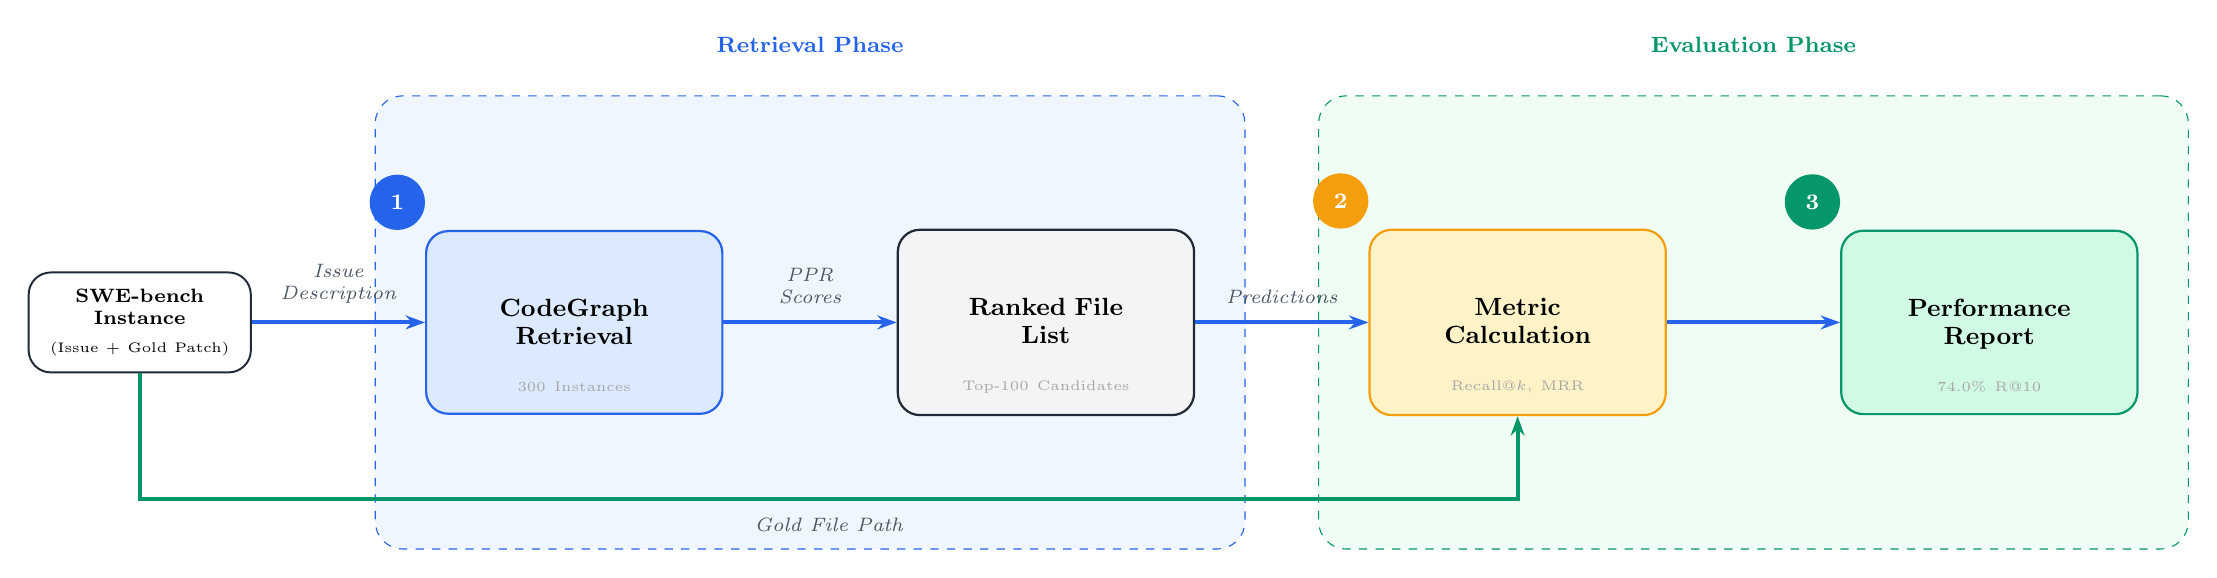
\begin{tikzpicture}[
            stage/.style={draw, rounded corners=8pt,
                    minimum width=3.6cm, minimum height=2.2cm,
                    text width=3.2cm, align=center,
                    line width=0.8pt, inner sep=8pt, font=\small},
            badge/.style={circle, minimum size=20pt, inner sep=0pt,
                    font=\footnotesize\bfseries, text=white, line width=0pt},
            datalabel/.style={font=\scriptsize\itshape, color={rgb,255:red,75;green,85;blue,99},
                    align=center, inner sep=2pt},
            arr/.style={-{Stealth[length=7pt, width=5pt]}, line width=1.5pt,
                    color={rgb,255:red,37;green,99;blue,235}},
            input/.style={draw, rounded corners=8pt, fill=white,
                    draw={rgb,255:red,31;green,41;blue,55}, line width=0.7pt,
                    font=\scriptsize, align=center, text width=2.4cm,
                    inner sep=6pt},
            node distance=2.2cm
        ]

        % ---------------------------------------------------------------
        % NODES
        % ---------------------------------------------------------------
        
        % Input: SWE-bench Instance
        \node[input] (instance) at (0,0) {\textbf{SWE-bench}\\\textbf{Instance}\\[2pt]\tiny (Issue + Gold Patch)};
        
        % Retrieval Stage
        \node[stage, fill={rgb,255:red,219;green,234;blue,254},
              draw={rgb,255:red,37;green,99;blue,235}, right=of instance] (retrieval)
            {\vspace{12pt}\\\textbf{CodeGraph}\\[-1pt]\textbf{Retrieval}\\[6pt]
             {\tiny\color{gray!70}300 Instances}};
             
        % Predictions
        \node[stage, fill={rgb,255:red,243;green,244;blue,246},
              draw={rgb,255:red,31;green,41;blue,55}, right=of retrieval] (topk)
            {\vspace{12pt}\\\textbf{Ranked File}\\[-1pt]\textbf{List}\\[6pt]
             {\tiny\color{gray!70}Top-100 Candidates}};

        % Validation Stage
        \node[stage, fill={rgb,255:red,254;green,243;blue,199},
              draw={rgb,255:red,245;green,158;blue,11}, right=of topk] (validation)
            {\vspace{12pt}\\\textbf{Metric}\\[-1pt]\textbf{Calculation}\\[6pt]
             {\tiny\color{gray!70}Recall@$k$, MRR}};

        % Performance Report
        \node[stage, fill={rgb,255:red,209;green,250;blue,229},
              draw={rgb,255:red,5;green,150;blue,105}, right=of validation] (report)
            {\vspace{12pt}\\\textbf{Performance}\\[-1pt]\textbf{Report}\\[6pt]
             {\tiny\color{gray!70}74.0\% R@10}};

        % Stage badges (Shifted to the top-left corner outside the box)
        \node[badge, fill={rgb,255:red,37;green,99;blue,235}]
            at ([xshift=-10pt,yshift=10pt]retrieval.north west) {\footnotesize 1};
        \node[badge, fill={rgb,255:red,245;green,158;blue,11}]
            at ([xshift=-10pt,yshift=10pt]validation.north west) {\footnotesize 2};
        \node[badge, fill={rgb,255:red,5;green,150;blue,105}]
            at ([xshift=-10pt,yshift=10pt]report.north west) {\footnotesize 3};

        % Arrows
        \draw[arr] (instance.east) -- node[datalabel, above, yshift=4pt] {Issue\\Description} (retrieval.west);
        \draw[arr] (retrieval.east) -- node[datalabel, above, yshift=4pt] {PPR\\Scores} (topk.west);
        \draw[arr] (topk.east) -- node[datalabel, above, yshift=4pt] {Predictions} (validation.west);
        \draw[arr] (validation.east) -- (report.west);
        
        % Gold File Path arrow
        \draw[arr, color={rgb,255:red,5;green,150;blue,105}] (instance.south) -- ++(0,-1.6) -| node[datalabel, pos=0.25, below, yshift=-4pt] {Gold File Path} (validation.south);

        % Phases
        \begin{scope}[on background layer]
            % Retrieval Phase
            \node[draw={rgb,255:red,37;green,99;blue,235}, dashed,
                  rounded corners=10pt,
                  fill={rgb,255:red,239;green,246;blue,255},
                  fit=(retrieval)(topk), inner xsep=18pt, inner ysep=48pt] (retphase) {};
            % Validation Phase
            \node[draw={rgb,255:red,5;green,150;blue,105}, dashed,
                  rounded corners=10pt,
                  fill={rgb,255:red,240;green,253;blue,244},
                  fit=(validation)(report), inner xsep=18pt, inner ysep=48pt] (valphase) {};
        \end{scope}
        
        \node[font=\footnotesize\bfseries, color={rgb,255:red,37;green,99;blue,235},
              above=12pt of retphase] {Retrieval Phase};
        \node[font=\footnotesize\bfseries, color={rgb,255:red,5;green,150;blue,105},
              above=12pt of valphase] {Evaluation Phase};

    \end{tikzpicture}%
    }
    \caption[SWE-bench Lite evaluation pipeline]{The evaluation pipeline for the SWE-bench Lite benchmark. For each instance, CodeGraph retrieves a ranked list of files based on the issue description, which the evaluation harness compares against the human-written gold patch to compute retrieval metrics.}
    \label{fig:eval-pipeline}
\end{figure}

% ------------------------------------------------------------
\subsection{Baselines}
\label{sec:eval-baselines}
% ------------------------------------------------------------

We compare CodeGraph against three baselines that together isolate the individual contributions of lexical matching, graph structure, and PPR ranking:
\begin{itemize}
    \item \textbf{Random:} Files are ranked uniformly at random. This establishes the performance floor and calibrates the absolute scale of improvements.
    \item \textbf{BM25-only:} A sparse lexical retriever over the same entity corpus used for seeds. This baseline shares CodeGraph's lexical foundation while omitting the structural component, making it the most important point of comparison for measuring the value of graph-based propagation.
    \item \textbf{One-hop ego graph:} An unranked structural baseline that returns all neighbours within one hop of the seed nodes. This tests whether graph structure alone, without a ranking function, provides useful retrieval signal.
\end{itemize}

All baselines run on the same SWE-bench Lite instances and repositories as CodeGraph, under the same evaluation protocol.

% ============================================================
\section{The Path to 74\% Retrieval Accuracy}
\label{sec:eval-trajectory}
% ============================================================

This section presents the performance trajectory from the initial baseline to the optimal configuration. The goal is to show not only where the system ended up, but how each engineering decision contributed to the final result, so that the trajectory itself serves as evidence for the design choices documented throughout this thesis.

The initial configuration, which uses confidence-weighted PPR restart, achieves 42.0\% R@10. For comparison, BM25 alone achieves 49.7\%, meaning the initial graph-based system underperforms a simple lexical baseline. This gap is the first key finding: it reveals that the problem lies not in the graph structure itself, but in how the personalization vector is constructed. The subsequent engineering iterations address this directly. \Cref{tab:trajectory-results} records the full trajectory.

\begin{table}[H]
    \centering
    \small
    \caption{Performance trajectory from the initial baseline to the optimal configuration. Each row adds one intervention to the previous configuration.}
    \label{tab:trajectory-results}
    \renewcommand{\arraystretch}{1.5}
    \begin{adjustbox}{max width=\textwidth}
    \begin{tabularx}{\textwidth}{@{} >{\RaggedRight\arraybackslash}X >{\RaggedRight\arraybackslash}p{1.2cm} >{\RaggedRight\arraybackslash}p{1.2cm} >{\RaggedRight\arraybackslash}p{1.2cm} >{\RaggedRight\arraybackslash}p{1.6cm} @{}}
        \toprule
        \textbf{Configuration} & \textbf{R@5} & \textbf{R@10} & \textbf{MRR} & \textbf{Zero-recall} \\
        \midrule
        Weighted PPR (Initial Baseline)  & 37.0\% & 42.0\% & 0.228 & 174 \\
        Uniform PPR (Algorithm Refinement) & 55.3\% & 60.7\% & 0.344 & 118 \\
        + Improved Seeds (Seed Engineering) & 60.7\% & 72.3\% & 0.439 & 83 \\
        + Top-$k$ = 30 (Final Optimal)      & \textbf{60.7\%} & \textbf{74.0\%} & \textbf{0.442} & \textbf{78} \\
        \midrule
        \textit{BM25-only Baseline}      & 37.7\% & 49.7\% & 0.248 & 151 \\
        \bottomrule
    \end{tabularx}
    \end{adjustbox}
\end{table}

The improvement trajectory follows three stages:
\begin{enumerate}
    \item \textbf{Algorithm Refinement (+18.7pp):} Switching from confidence-weighted to uniform PPR restart closes the gap with BM25 and immediately surpasses it. When seeds are noisy or ambiguous, assigning them proportional weights amplifies false positives and misdirects the random walk. Uniform restart lets graph topology resolve the competition between seeds, which is more reliable than seed confidence scores.
    \item \textbf{Seed Engineering (+11.6pp):} Implementing compound tokenization, an expanded BM25 corpus, and inverse-frequency weighting ensures that natural-language issue descriptions can be mapped to code entities reliably. This is the most impactful engineering intervention across all iterations.
    \item \textbf{Budget Adjustment (+1.7pp):} Increasing the candidate pool from $k=20$ to $k=30$ recovers a small band of instances where PPR correctly identified the target neighbourhood but ranked the gold file just outside the initial threshold.
\end{enumerate}

\begin{figure}[H]
    \centering
    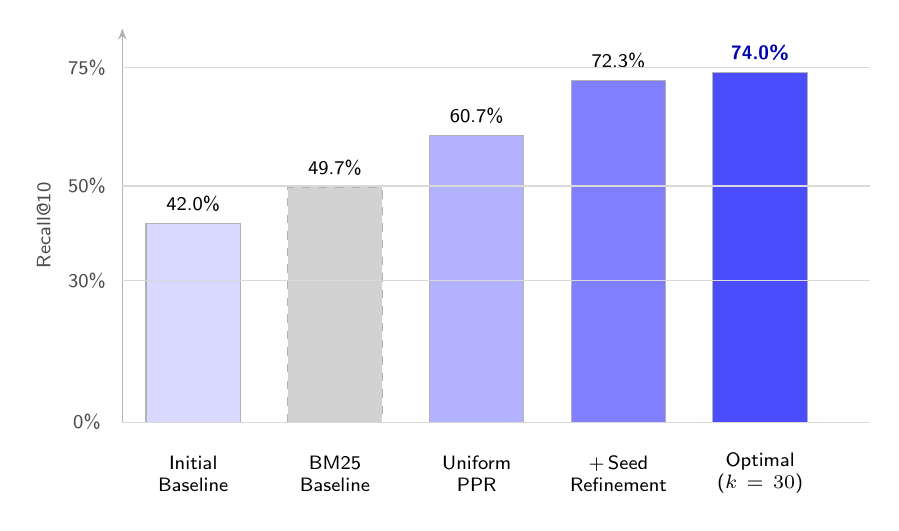
\begin{tikzpicture}[
            lbl/.style={font=\scriptsize\sffamily, align=center},
        ]
        \pgfmathsetmacro{\hA}{42.0*0.06}
        \pgfmathsetmacro{\hB}{49.7*0.06}
        \pgfmathsetmacro{\hC}{60.7*0.06}
        \pgfmathsetmacro{\hD}{72.3*0.06}
        \pgfmathsetmacro{\hE}{74.0*0.06}

        \fill[blue!15, draw=gray!60] (0,   0) rectangle (1.2, \hA);
        \fill[gray!35, draw=gray!60, dashed] (1.8, 0) rectangle (3.0, \hB);
        \fill[blue!30, draw=gray!60] (3.6, 0) rectangle (4.8, \hC);
        \fill[blue!50, draw=gray!60] (5.4, 0) rectangle (6.6, \hD);
        \fill[blue!70, draw=gray!60] (7.2, 0) rectangle (8.4, \hE);

        \node[lbl] at (0.6,  \hA+0.25) {42.0\%};
        \node[lbl] at (2.4,  \hB+0.25) {49.7\%};
        \node[lbl] at (4.2,  \hC+0.25) {60.7\%};
        \node[lbl] at (6.0,  \hD+0.25) {72.3\%};
        \node[lbl, text=blue!70!black, font=\scriptsize\sffamily\bfseries] at (7.8,  \hE+0.25) {74.0\%};

        \node[lbl, text width=1.6cm] at (0.6,  -0.65) {Initial\\Baseline};
        \node[lbl, text width=1.6cm] at (2.4,  -0.65) {BM25\\Baseline};
        \node[lbl, text width=1.6cm] at (4.2,  -0.65) {Uniform\\PPR};
        \node[lbl, text width=1.8cm] at (6.0,  -0.65) {+\,Seed\\Refinement};
        \node[lbl, text width=1.6cm] at (7.8,  -0.65) {Optimal\\($k=30$)};

        \draw[-{Stealth[length=4pt]}, gray!60, semithick] (-0.3, 0) -- (-0.3, 5.0);
        \node[rotate=90, lbl, text=gray!60!black] at (-1.3, 2.5) {Recall@10};
        \foreach \y/\pct in {0/0, 1.8/30, 3.0/50, 4.5/75} {
            \draw[gray!30, thin] (-0.3, \y) -- (9.2, \y);
            \node[lbl, text=gray!60!black] at (-0.75, \y) {\pct\%};
        }
    \end{tikzpicture}
    \caption{Recall@10 trajectory. We show the grey bar (BM25-only) for reference; the remaining bars represent successive CodeGraph configurations.}
    \label{fig:trajectory}
\end{figure}

% ============================================================
\section{The Reachability Bottleneck}
\label{sec:eval-diagnostics}
% ============================================================

This section explains the diagnostic insight that motivated the Seed-First engineering strategy. Understanding why failures occur is more informative than knowing how many occur: this analysis reveals that CodeGraph's retrieval ceiling is set by a structural property of the dependency graph, not by the ranking function.

\paragraph{The Bimodal Rank Distribution.}
When we inspected the distribution of ranks for the target file across the initial configuration, we found a striking bimodal pattern: for most issues, the target file either ranks in the top-5 or does not appear in the top-10 at all. Only 15 out of 300 instances (5\%) fall in the intermediate band (ranks 6--10). This pattern holds across configurations and repositories, and is illustrated in \cref{fig:bimodal}.

\paragraph{What the Bimodal Pattern Reveals.}
The near-absence of intermediate ranks implies that PPR ranking is not the primary bottleneck. When the system retrieves the gold file at all, it almost always ranks it highly: the ranking function is working correctly. The dominant failure mode is Reachability: if no seed lies on a structurally connected path to the target file, PPR has no signal to propagate there, and the target does not appear in the output regardless of how the ranking is configured.

The 15 intermediate cases (ranks 6--10) represent a distinct secondary effect: these typically involve dense modules where probability mass is distributed across many related files, or utility-function paths where IDF reweighting reduces but does not eliminate the spreading of relevance across semantically unrelated neighbours.

This diagnostic directly motivates the Seed-First engineering strategy described in \cref{sec:eval-seeds}. If the ceiling is set by Reachability, the highest-leverage intervention is improving seed quality, not refining the ranking algorithm. \Cref{tab:attribution-summary} quantifies this attribution.

\begin{table}[H]
    \centering
    \small
    \caption{Attribution of performance gains to engineering interventions. Seed quality is the primary driver of retrieval success.}
    \label{tab:attribution-summary}
    \renewcommand{\arraystretch}{1.5}
    \begin{adjustbox}{max width=\textwidth}
    \begin{tabularx}{\textwidth}{@{} >{\RaggedRight\arraybackslash}p{4.2cm} >{\RaggedRight\arraybackslash}X >{\RaggedRight\arraybackslash}p{1.4cm} @{}}
        \toprule
        \textbf{Factor} & \textbf{Intervention} & \textbf{$\Delta$R@10} \\
        \midrule
        Algorithm Refinement    & Uniform vs. weighted PPR restart   & +18.7pp \\
        Seed Quality Refinement & Compound tokenization, IDF weighting & +11.6pp \\
        Budget Adjustment       & Candidate pool $k=30$ & +1.7pp \\
        \midrule
        \textbf{Total Improvement} & & \textbf{+32.0pp} \\
        \bottomrule
    \end{tabularx}
    \end{adjustbox}
\end{table}

\begin{figure}[H]
    \centering
    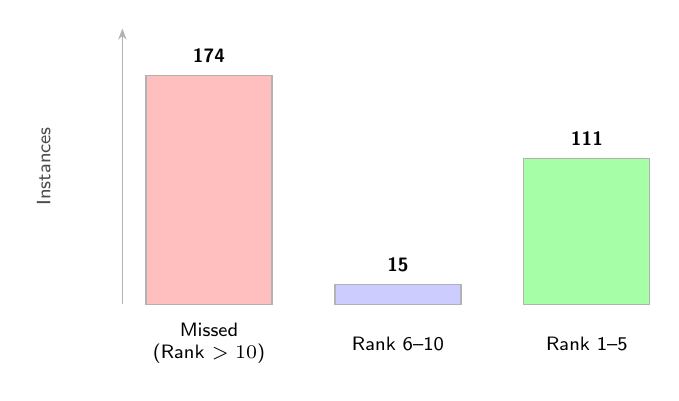
\begin{tikzpicture}[
            lbl/.style={font=\scriptsize\sffamily, align=center},
        ]
        % Heights proportional to instance counts (174, 15, 111 out of 300)
        \pgfmathsetmacro{\hMissed}{174/300*5}
        \pgfmathsetmacro{\hMid}{15/300*5}
        \pgfmathsetmacro{\hTop}{111/300*5}
        \fill[red!25, draw=gray!60] (0, 0) rectangle (1.6, \hMissed);
        \fill[blue!20, draw=gray!60] (2.4, 0) rectangle (4.0, \hMid);
        \fill[green!35, draw=gray!60] (4.8, 0) rectangle (6.4, \hTop);
        \node[lbl] at (0.8, \hMissed+0.25) {\textbf{174}};
        \node[lbl] at (3.2, \hMid+0.25) {\textbf{15}};
        \node[lbl] at (5.6, \hTop+0.25) {\textbf{111}};
        \node[lbl] at (0.8, -0.5) {Missed\\(Rank $>10$)};
        \node[lbl] at (3.2, -0.5) {Rank 6--10};
        \node[lbl] at (5.6, -0.5) {Rank 1--5};
        \draw[-{Stealth[length=4pt]}, gray!60, semithick] (-0.3, 0) -- (-0.3, 3.5);
        \node[rotate=90, lbl, text=gray!60!black] at (-1.3, 1.75) {Instances};
    \end{tikzpicture}
    \caption{Bimodal rank distribution for the initial configuration (300 instances). Instances land almost exclusively in Rank 1--5 or outside the top~10; only 5\% fall in the intermediate band. This pattern implies that PPR ranking is not the primary bottleneck once a useful seed exists.}
    \label{fig:bimodal}
\end{figure}

% ============================================================
\section{Systematic Seed Refinement}
\label{sec:eval-seeds}
% ============================================================

The diagnostic finding that Reachability sets the retrieval ceiling establishes a clear engineering principle: improving seed quality is more effective than improving the ranking function. This section details the five interventions that implement this Seed-First strategy.

\begin{enumerate}
    \item \textbf{Uniform PPR Restart (Algorithm Alignment):} The initial configuration assigns restart probabilities proportional to seed confidence scores, meaning a few high-confidence but lexically ambiguous matches can dominate the personalization vector and misdirect the random walk. Switching to a uniform restart distribution gives each seed an equal share of restart mass and lets graph topology resolve the competition between seeds. This is the most impactful single change in the trajectory (+18.7pp).

    \item \textbf{Compound Tokenization (Lexical Recovery):} Standard lexical indexing treats identifiers as atomic tokens. A query containing the word ``compiler'' does not match an entity named \texttt{SQLCompiler} because the two strings are lexically distinct. Compound tokenization decomposes camel-case and underscore-separated identifiers into their constituent terms before indexing: \texttt{SQLCompiler} becomes \{sql, compiler\}. This allows issue descriptions to resolve to compound code identifiers that would otherwise remain invisible to the lexical index.

    \item \textbf{Expanded BM25 Corpus (Contextual Scope):} The initial BM25 index covers only docstrings and function bodies. We expand it to include file paths, class names, and qualified method names. Issue descriptions frequently name modules or packages by their directory path rather than by any function inside them, so indexing file paths allows these references to resolve to structural seeds.

    \item \textbf{Inverse-Frequency Entity Weighting (Noise Reduction):} Not all matched entities are equally informative as seeds. A match on \texttt{update} or \texttt{save} tells us very little about which part of the codebase is relevant, because these names appear in dozens of files. We weight seeds by the inverse document frequency of their names: entities with rare names receive higher weight than entities with common names. This penalizes uninformative seeds without discarding them entirely.

    \item \textbf{Candidate Budget Optimization ($k=30$):} The initial configuration returns the top-20 ranked files. Increasing this to 30 recovers 5 instances where PPR correctly identified the target neighbourhood but ranked the gold file between positions 21 and 30. The cost of returning 10 additional files per query is a minor increase in context, not a meaningful increase in latency.
\end{enumerate}

Together, these five interventions implement a coherent engineering strategy: reduce lexical mismatch between issue descriptions and code identifiers, amplify informative seeds while suppressing ambiguous ones, and let graph topology propagate structural relevance. \Cref{sec:eval-ablations} validates each component through controlled ablations.

% ============================================================
\section{Ablation Studies and Architectural Validation}
\label{sec:eval-ablations}
% ============================================================

This section justifies our design decisions through controlled ablation studies. Each experiment isolates a design component, measures its individual contribution to the final retrieval accuracy, and provides empirical evidence for the choices made throughout this thesis.

% ------------------------------------------------------------
\subsection{Algorithm Selection: Uniform vs. Weighted Restart}
\label{sec:eval-ablation-algorithm}
% ------------------------------------------------------------

The most consequential algorithmic choice is the restart distribution for Personalized PageRank. In the initial configuration, restart probabilities are proportional to the confidence scores of retrieved seeds: a highly confident but lexically common seed (such as a function named \texttt{update} found in dozens of files) dominates the personalization vector and directs most probability mass toward a generic part of the graph.

Switching to uniform restart raises R@10 from 42.0\% to 60.7\%, a gain of 18.7 percentage points. When seeds are ambiguous, weighting by confidence amplifies false positives, while uniform restart lets structural graph connectivity determine where probability accumulates. This result is consistent with the bimodal observation in \cref{sec:eval-diagnostics}: the ranking function works correctly when given a useful starting point; the bottleneck is the quality of that starting point, not how the probabilities are spread.

% ------------------------------------------------------------
\subsection{Hyperparameter Sensitivity: Budget and Damping}
\label{sec:eval-ablation-tuning}
% ------------------------------------------------------------

We sweep over the candidate budget $k$ and the PPR damping factor $\alpha$ to characterize the sensitivity of the optimal configuration.

\begin{itemize}
    \item \textbf{Candidate Budget ($k$):} Increasing $k$ from 20 to 30 yields 1.7pp. Increasing further to 50 provides no additional gain, confirming that the marginal benefit of a larger candidate pool falls off quickly once the structurally reachable neighbourhood is covered.
    \item \textbf{Damping Factor ($\alpha$):} We test values from 0.10 to 0.85. The system is robust across a wide range, with performance stable between $\alpha=0.55$ and $\alpha=0.80$. The chosen value of $\alpha=0.70$ performs consistently across all 12 repositories. Lower values cause over-spreading: probability mass diffuses too broadly and the ranking loses discrimination. Higher values confine the random walk to the immediate neighbourhood of the seeds, which limits PPR's ability to reach structurally adjacent modules.
\end{itemize}

% ------------------------------------------------------------
\subsection{Graph Schema: Validation via Co-location Edges}
\label{sec:eval-ablation-structural}
% ------------------------------------------------------------

To test the limits of the graph schema, we explore augmenting the existing edge types (CALLS, IMPORTS, CONTAINS, INHERITS\_FROM) with \texttt{CO\_LOCATED} edges that connect all sibling files within the same directory. The intuition is that files sharing a directory often collaborate, and adding these edges might allow PPR to propagate relevance within a directory without requiring an explicit import.

The result is a regression of 1.0 percentage point. In large, functionally heterogeneous directories such as \texttt{django/\allowbreak db/\allowbreak models/}, the new edges create a dense subgraph connecting unrelated files. PPR probability mass spreads across this subgraph indiscriminately (Probability Dilution), and the original ranked files are displaced by irrelevant neighbours.

This experiment validates the final schema. CodeGraph's precision derives from dependency-based edges that encode real structural relationships, not from proximity-based heuristics. Artificial graph expansion introduces noise that the ranking function cannot distinguish from genuine structural evidence, and the optimal configuration therefore prioritizes high-fidelity Seed Extraction over structural density.

% ============================================================
\section{Qualitative Synthesis and Structural Limits}
\label{sec:eval-synthesis}
% ============================================================

The quantitative trajectory in \cref{sec:eval-trajectory} shows how far the system improved. This section explains where it does well, where it struggles, and why. Understanding the structural limits of CodeGraph is as important for the thesis argument as reporting the headline metric.

\paragraph{Codebase Structure and Retrieval Success.}
\Cref{tab:per-repo} shows zero-recall failure rates for the five most-represented repositories. Performance varies considerably, and the variation is explained by two structural properties of each codebase: module cohesion and directory density.

\begin{table}[H]
    \centering
    \small
    \caption{Zero-recall failure rates by repository for the optimal configuration.}
    \label{tab:per-repo}
    \renewcommand{\arraystretch}{1.4}
    \begin{adjustbox}{max width=\textwidth}
    \begin{tabularx}{\textwidth}{@{} >{\RaggedRight\bfseries}p{4.2cm} >{\RaggedRight\arraybackslash}X >{\RaggedRight\arraybackslash}X >{\RaggedRight\arraybackslash}X @{}}
        \toprule
        \textbf{Repository} & \textbf{Instances} & \textbf{Zero-recall} & \textbf{Failure rate} \\
        \midrule
        scikit-learn      & 23 & 2  & 9\%  \\
        matplotlib        & 23 & 3  & 13\% \\
        django/django     & 114 & 31 & 27\% \\
        sympy/sympy       & 77 & 24 & 31\% \\
        pylint-dev/pylint & 6  & 5  & 83\% \\
        \midrule
        \textbf{Total (Weighted Avg)} & \textbf{300} & \textbf{78} & \textbf{26\%} \\
        \bottomrule
    \end{tabularx}
    \end{adjustbox}
\end{table}

\noindent The system achieves near-perfect recall on scikit-learn (9\% failure rate) and matplotlib (13\%). Both repositories feature distinct subpackages with clear, non-overlapping domains. When a bug report mentions a concept from one subpackage, BM25 selects precise seeds and PPR amplifies them within a cohesive module cluster that contains the relevant file.

Django (27\% failure rate) and SymPy (31\%) present more difficulty. Both contain large, functionally heterogeneous directories where a single directory mixes logically distinct concerns. In \texttt{django/\allowbreak db/\allowbreak models/}, for example, more than 25 files span ORM query generation, model field validation, and migration management. When a seed lands in this directory, it has no explicit IMPORTS or CALLS edge to a specific sibling file, so PPR cannot propagate relevance within the directory.

pylint-dev/pylint (83\% failure rate) is an outlier with only 6 instances. Pylint's architecture is plugin-driven: the relevant file for a given bug is often a plugin module registered dynamically rather than imported explicitly. Static dependency analysis cannot extract these edges, so the graph for these instances is structurally disconnected from the relevant files.

\paragraph{The Structural Failure Taxonomy.}
An analysis of the 78 zero-recall instances identifies two distinct failure modes that together define the structural boundary of graph-based retrieval. \Cref{fig:taxonomy} organizes them.

\begin{figure}[H]
    \centering
    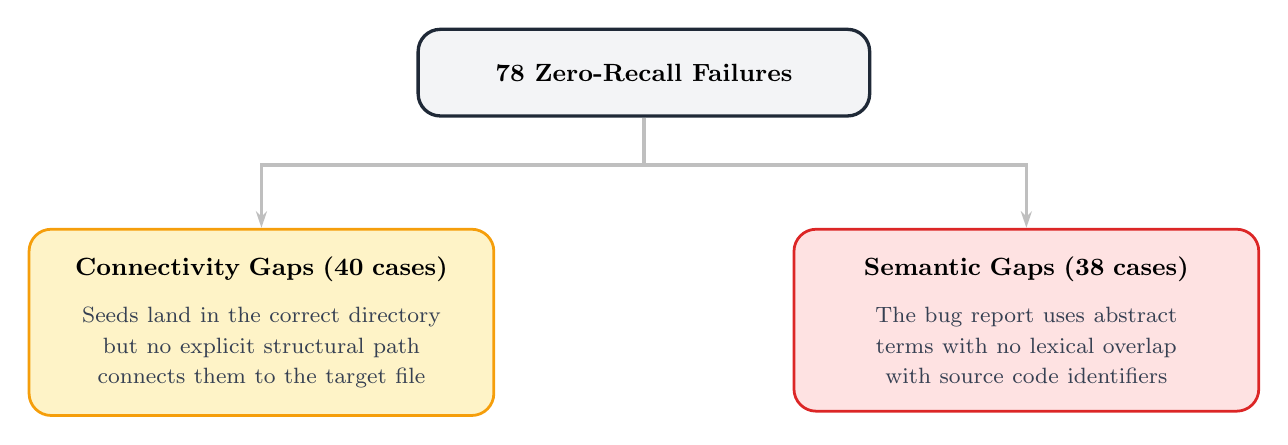
\begin{tikzpicture}[
        node distance=2.0cm and 0.5cm,
        rootbox/.style={draw, rounded corners=8pt, line width=1.2pt,
            fill={rgb,255:red,243;green,244;blue,246},
            draw={rgb,255:red,31;green,41;blue,55},
            text width=5.5cm, align=center, font=\small\bfseries, minimum height=1.1cm},
        leafbox/.style={draw, rounded corners=8pt, line width=1.0pt,
            text width=5.2cm, align=center, font=\small, minimum height=1.6cm,
            inner sep=10pt},
        arrow/.style={-{Stealth[length=6pt, width=4pt]}, line width=1.2pt, color=gray!50},
        subtextstyle/.style={font=\footnotesize, color={rgb,255:red,55;green,65;blue,81}, 
            line height=1.25},
    ]
    \newcommand{\subtext}[1]{{\color[rgb]{0.21,0.25,0.32}\footnotesize #1}}
        % Root
        \node[rootbox] (total) {78 Zero-Recall Failures};
        
        % Connectivity Gaps
        \node[leafbox, fill={rgb,255:red,254;green,243;blue,199}, 
              draw={rgb,255:red,245;green,158;blue,11}, below left=1.4cm and -1.0cm of total] (connectivity) 
            {\textbf{Connectivity Gaps (40 cases)}\\[6pt]
             \subtext{Seeds land in the correct directory but no explicit structural path connects them to the target file}};
             
        % Semantic Gaps
        \node[leafbox, fill={rgb,255:red,254;green,226;blue,226}, 
              draw={rgb,255:red,220;green,38;blue,38}, below right=1.4cm and -1.0cm of total] (semantic) 
            {\textbf{Semantic Gaps (38 cases)}\\[6pt]
             \subtext{The bug report uses abstract terms with no lexical overlap with source code identifiers}};
        
        % Arrows
        \draw[arrow] (total.south) -- ++(0,-0.6) -| (connectivity.north);
        \draw[arrow] (total.south) -- ++(0,-0.6) -| (semantic.north);

    \end{tikzpicture}
    \caption{Failure taxonomy of the 78 zero-recall instances. Connectivity Gaps account for 40 cases and arise from missing structural paths in the dependency graph. Semantic Gaps account for 38 cases and arise from lexical mismatch between issue descriptions and source code identifiers.}
    \label{fig:taxonomy}
\end{figure}

\begin{itemize}
    \item \textbf{Connectivity Gaps (40 instances):} These occur when seeds land in the correct part of the codebase (the correct directory, or a file that calls into the relevant module) but no explicit CALLS or IMPORTS edge connects them to the specific target file. Without such a path, Personalized PageRank cannot propagate relevance to the target, regardless of seed quality. This failure mode reflects the inherent limitation of static dependency analysis: files that are logically related but not structurally connected through explicit edges are invisible to graph propagation.

    \item \textbf{Semantic Gaps (38 instances):} These failures arise when the issue description uses abstract natural-language terms with no lexical overlap with any identifier in the source code. A bug described as ``the ORM silently discards null values during bulk insertion'' does not contain the identifier \texttt{bulk\_create} or \texttt{\_do\_insert}. Without a lexical match, the BM25 stage cannot place any seed in the relevant neighbourhood, and PPR has no starting point. This failure mode requires semantic understanding beyond what a lexical index can provide.
\end{itemize}

\paragraph{Conclusion.}
These two failure modes define the structural ceiling of the CodeGraph approach. Connectivity Gaps arise from the sparsity of explicit dependency edges across logically related files. Semantic Gaps arise from the inability of lexical matching to bridge abstract bug descriptions to code identifiers. Both are addressable in principle: Connectivity Gaps through richer graph schemas (with the caveat from \cref{sec:eval-ablation-structural} that naive structural augmentation introduces Probability Dilution), and Semantic Gaps through dense embedding retrieval that connects natural-language descriptions to code entities through learned similarity. The integration of these two retrieval modalities is the primary direction for future work, discussed further in \cref{ch:conclusion}.


\bibliography{references}

\end{document}
